\chapter{Espacios Recubridores}

\begin{observacion}
    A lo largo de este tema supondremos que todos los espacios topológicos son conexos y localmente arcoconexos. En particular estos espacios son siempre arcoconexos.
\end{observacion}

\section{Levantamiento de aplicaciones}

\begin{observacion}
    Vamos a tener en cuenta que si $X$ es un espacio topológico conexo y localmente arcoconexo, entonces todo abierto suyo cumple que cada componente arcoconexa es abierta.

    \begin{proof}
        Si $O$ es abierto y $A$ es una componente arcoconexa de $O$, entonces dado $a\in A$, como $X$ es localmente arcoconexo tendremos que existe un $U$ entorno arcoconexo de $a$ tal que $U\subseteq O$. Como $A$ es el mayor arcoconexo en $O$ que contiene al punto $a$ tendremos que $U\subseteq A$, luego $A$ es abierto.
    \end{proof}
    
    Esto lo vamos a usar para el caso en el que tenemos dada una aplicación recubridora $p:R\to B$ y un punto $b_0\in B$. Entonces tendremos que existe un abierto regularmente recubierto $O$ que contiene a $b_0$. Restringiéndonos a la componente arcoconexa de $O$ que contiene a $b_0$ podremos suponer que el entorno regularmente recubierto es abierto y arcoconexo.
\end{observacion}

\begin{lema}[Unicidad del levantamiento]
    Sean $p:R \to B$ una aplicación recubridora, $f_1,f_2:X\to R$ continuas tales que 
    \begin{gather*}
        p\circ f_1 = p\circ f_2
    \end{gather*}
    Si existe un $x_0\in X$ tal que $f_1(x_0)=f_2(x_0)$, entonces $f_1=f_2$.

    \begin{proof}
        Para la demostración solo se necesita que $X$ sea conexo y no necesariamente localmente arcoconexo. \\

        Partimos de la siguiente situación
        \begin{gather*}
            \xymatrix{
                && R \ar[d]^{p}\\
                X \ar[urr]^{f_1,f_2} \ar[rr]_{f=p\circ f_1 = p\circ f_2} && B
            }
        \end{gather*}
        Consideramos el siguiente conjunto
        \begin{gather*}
            Y=\{x\in X : f_1(x)=f_2(x)\}
        \end{gather*}
        Como $X$ es conexo y tenemos que $Y \neq \emptyset$, ya que por hipótesis $x_0\in Y$, si probamos que $Y$ es abierto y cerrado tendremos que $Y=X$, es decir, $f_1=f_2$. \\
        
        Veamos que $Y$ es abierto. Para ello tomamos $y\in Y$, es decir, un punto $y$ tal que $f_1(y)=f_2(y)$. Elegimos el punto $b=p(f_1(y))=p(f_2(y))$. Sea $O$ abierto regularmente recubierto y arcoconexo que contiene a $b$, entonces 
        \begin{gather*}
            p^{-1}(O) = \bigcup\limits_{i\in I} A_i
        \end{gather*}
        donde los $A_i$ son abiertos disjuntos de $R$ y tal que 
        \begin{gather*}
            p_{|A_i}: A_i \to O
        \end{gather*} 
        es un homeomorfismo. Tomamos el abierto $A_{i_0}$ donde se encuentra $f_1(y)=f_2(y)$. Elegimos $V=f_1^{-1}(A_{i_0}) \cap f_2^{-1}(A_{i_0})$. Veamos que $\forall x \in V$ se tiene que $f_1(x)=f_2(x)$. Como $x\in V$ tendremos que $f_1(x),f_2(x)\in A_{i_0}$ por lo que 
        \begin{gather*}
            p(f_1(x)) = p(f_2(x)) \overset{(\ast)}{\Rightarrow} f_1(x)=f_2(x) \Rightarrow V\subseteq Y
        \end{gather*}
        donde en $(\ast)$ hemos usado que $p_{|A_i}$ es inyectiva. Tenemos finalmente que $Y$ es abierto.\\

        Veamos ahora que $Y$ es cerrado. Para ello demostramos que $X\setminus Y$ es abierto. Tomamos $y\in X\setminus Y$ y vemos que existe un $V$ abierto que contiene al punto $y$ y tal que $V\subseteq X \setminus Y$. Sea $b=p(f_1(y))=p(f_2(y))$ y de nuevo tomamos $O$ regularmente recubierto que contiene a $b$. Tendremos
        \begin{gather*}
            p^{-1}(O) = \bigcap\limits_{i\in I} A_i
        \end{gather*}
        donde los $A_i$ son abiertos disjuntos y tal que 
        \begin{gather*}
            p_{|A_i}: A_i\to O 
        \end{gather*}
        es un homeomorfismo. Tendremos $f_1(y)\in A_{i_1}$ y $f_2\in A_{i_2}$ y además se verificará que $A_{i_1}\neq A_{i_2}$ ya que si se diera la igualdad tendríamos que la aplicación
        \begin{gather*}
            p_{|A_{i_1}}: A_{i_1} \to O
        \end{gather*}
        no sería intectiva. Elegimos ahora $V=f_1^{-1}(A_1) \cap f_2^{-1}(A_2)$, donde se tiene que $y\in V$. Además se tiene que 
        \begin{gather*}
            f_1(V)\subseteq A_{i_1}\\
            f_2(V)\subseteq A_{i_2}
        \end{gather*}
        por lo que para cada $x\in V$ se tendrá que $f_1(x)\neq f_2(x)$ ya que $f_1(x)\in A_{i_1}$ y $f_2(x)\in A_{i_2}$. Esto nos dice que $V\subseteq X\setminus Y$, luego $Y$ es cerrado.
    \end{proof}
\end{lema}

\begin{teo}[Teorema de monodromía]
    Sean $p:R \to B$ una aplicación recubridora, $b_0\in B$ y $r_0\in p^{-1}(b_0)$. El homomorfismo inducido $p_*:\pi_1(R,r_0)\to \pi_1(B,b_0)$ es inyectivo. En partircular, $\pi_1(R,r_0)$ es isomorfo a $p_*(\pi_1(R,r_0))< \pi_1(B,b_0)$.

    \begin{proof}
        Sabemos que $p_*$ es inyectiva si y solo si $\ker(p_*)$ es trivial. Tomamos $\alpha$ lazo basado en $r_0$ tal que 
        \begin{gather*}
            p_*([\alpha]) = [\veps_{b_0}]
        \end{gather*}
        Como además $[p\circ \alpha] = p^*([\alpha])$ tenemos que existe una homotopía por lazos de $\veps_{b_0}$ en $p\circ \alpha$. Como toda homotopía por arcos se puede levantar tenemos que existe una homotopía por arcos en $R$ de $\hat{\veps}_{b_0}$ y $\widehat{p\circ \alpha}$ (empezando en $r_0$). Tenemos
        \begin{gather*}
            \left.
            \begin{array}{l}
                \hat{\veps}_{b_0} = \veps_{r_0}\\\\
                \widehat{p\circ \alpha} = \alpha
            \end{array}
            \right\}  \Rightarrow [\alpha] = [\veps_{r_0}]
        \end{gather*}
    \end{proof}
\end{teo}

\begin{observacion}
    Recordemos que dados dos subgrupos $H_1,H_2$ de un grupo $G$ se dice que $H_1$ y $H_2$ son conjugados si existe un $g\in G$ tal que 
    \begin{gather*}
        H_2=g^{-1}H_1 g
    \end{gather*}
\end{observacion}

\begin{coro}
    Sean $p:R \to B$ una aplicación recubridora, $b_0\in B$ y $r_1,r_2\in p^{-1}(b_0)$. Elegimos un arco $\alpha:[0,1]\to R$ tal que
    \begin{gather*}
        \alpha(0)=r_1\\
        \alpha(1)=r_2
    \end{gather*}
    entonces 
    \begin{gather*}
        p_*(\pi_1(R,r_2)) = [p\circ\alpha]^{-1} \ast p_*(\pi_1(R,r_1)) \ast [p\circ\alpha]
    \end{gather*}
    En particular, $p_*(\pi_1(R,r_1))$ y $p_*(\pi_1(R,r_2))$ son conjugados en $\pi_1(B,b_0)$.

    \begin{proof}
        Sabemos que $p\circ \alpha$ es un lazo basado en $b_0$ por lo que $[p\circ \alpha]\in \pi_1(B,b_0)$. Además,
        \begin{align*}
            \pi_1(R,r_2) &\overset{isom.}{\longrightarrow} \pi_1(R,r_1)\\
            [\beta] &\longmapsto [\alpha \ast \beta \ast \tilde{\alpha}]
        \end{align*}
        Tenemos por tanto que 
        \begin{gather*}
            \pi_1(R,r_1) = [\alpha] \ast \pi_1(R,r_2) \ast [\tilde{\alpha}]\\
            p_*(\pi_1(R,r_1)) = [p\circ \alpha] \ast p_*(\pi_1(R,r_2)) \ast [p\circ \tilde{\alpha}]
        \end{gather*}
        Como tenemos que 
        \begin{gather*}
            [p\circ \tilde{\alpha}] = [\tilde{p\circ \alpha}] = [p\circ \alpha]^{-1}
        \end{gather*}
        llegamos a que son conjugados.
    \end{proof}
\end{coro}

\begin{coro}
    Sean $p:R\to B$ una aplicación recubridora, $b_0\in B$ y $r_1\in p^{-1}(b_0)$. Sea $H$ un subgrupo conjugado de $p_*(\pi_1(R,r_1))$ en $\pi_1(B,b_0)$. Entonces existe un punto $r_2\in R$ tal que
    \begin{gather*}
        H=p_*(\pi_1(R,r_2))
    \end{gather*}
    \begin{proof}
        Por hipótesis sabemos que $p(r_1)=b_0$ y que $p_*(\pi_1(R,r_1))$ es conjugado con $H$ en $\pi_1(B,b_0)$, es decir, 
        \begin{gather*}
            H = g^{-1} \ast p_*(\pi_1(R,r_1)) \ast g
        \end{gather*}
        con $g\in \pi_1(B,b_0)$, esto es, $g=[\gamma]$. Consideramos $\hat{\gamma}$ el levantamiento de $\gamma$ a $R$ con 
        \begin{gather*}
            \hat{\gamma}(0) = r_1
        \end{gather*}
        y llamamos $r_2=\hat{\gamma}(1)$ al final del arco.
        \begin{gather*}
            p(r_2) = (p\circ \hat{\gamma})(1) = \gamma(1) = b_0
        \end{gather*}
        Usando el corolario anterior tenemos que 
        \begin{align*}
            p_*(\pi_1(R,r_2)) &= [p\circ \hat{\gamma}]^{-1} \ast p_*(\pi_1(R,r_1)) \ast [p\circ \hat{\gamma}] =\\
            &= [\gamma]^{-1} \ast p_*(\pi_1(R,r_1)) \ast [\gamma] =\\
            &= H
        \end{align*}
    \end{proof}
\end{coro}

\begin{teo}
    Consideramos una aplicación recubridora $p:R\to B$, una aplicación continua $f:X\to B$, $x_0\in X$, $b_0=f(x_0)$ y $r_0\in p^{-1}(b_0)$. 
    
    \begin{gather*}
        \xymatrix{
            & R \ar[d]^p\\
            X \ar[r]^{f} \ar@{-->}[ur]^{\hat{f}} & B
        }
    \end{gather*}

    Entonces son equivalentes:
    \begin{enumerate}
        \item Existe un levantamiento $\hat{f}:X \to R$ de $f$ con $\hat{f}(x_0)=r_0$.
        \item $f_*(\pi_1(X,x_0))\subseteq p_*(\pi_1(R,r_0))$
    \end{enumerate}
    Además, si se cumple cualquiera de estas condiciones, el levantamiento $\hat{f}$ de $f$ con $\hat{f}(x_0)=r_0$ es único.

    \begin{proof}\
        \begin{itemize}
            \item [(1) $\Rightarrow$ (2)] Estamos en la situación del siguiente diagrama
            \begin{gather*}
                \xymatrix{
                    & \pi_1(R,r_0) \ar[d]^{p_*}\\
                    \pi_1(X,x_0) \ar[ur]^{\hat{f}_*} \ar[r]_{f_*} & \pi_1(B,b_0)
                }
            \end{gather*}
            y podemos ver que 
            \begin{gather*}
                f_*(\pi_1(X,x_0)) = p_*(\hat{f}_*(\pi_1(X,x_0))) \subseteq p_*(\pi_1(R,r_0))
            \end{gather*}
            ya que $\hat{f}_*(\pi_1(X,x_0))\subseteq \pi_1(R,r_0)$ por lo que tenemos esta implicación simplemente desarrollando la composición.

            \item [(2) $\Rightarrow$ (1)] Empezamos definiendo $\hat{f}$:
            \begin{gather*}
                \xymatrix{
                    & R \ar[d]^p\\
                    X \ar[r]^f & B
                }
            \end{gather*}
            Dado $x\in X$ elegimos $\alpha_x$ un arco en $X$ que una $x_0$ con $x$. Entonces $f\circ \alpha_x$ es un arco en $B$ que une $b_0 = f(x_0)$ con $f(x)$. Consideramos ahora $\widehat{f\circ \alpha_x}$ el único arco en $R$ tal que $\widehat{f\circ \alpha_x}(0) = r_0$ y definimos 
            \begin{gather*}
                \hat{f}(x) = \widehat{f\circ \alpha_x}(1)
            \end{gather*}
            Veamos que $\hat{f}$ está bien definida, es decir, que no depende del arco $\alpha_x$ elegido. Tomamos otro arco $\beta_x$ en $X$ tal que $\beta_x(0)=x_0$ y $\beta_x(1)=x$ y queremos ver que
            \begin{gather*}
                \widehat{f\circ \alpha_x}(1) = \widehat{f\circ \beta_x}(1)
            \end{gather*}

            Tomamos $\gamma=\alpha_x \ast \tilde{\beta_x}$ que es un lazo en $X$ con base en $x_0$. Tenemos entonces que 
            \begin{gather*}
                f \circ \gamma = (f\circ \alpha_x) \ast (f \circ \tilde{\beta_x})
            \end{gather*}
            es un lazo con base en $b_0$. Usamos ahora la hipótesis y tenemos que 
            \begin{gather*}
                [f\circ \gamma] = f_*([\gamma]) \in p_*(\pi_1(R, r_0))
            \end{gather*}
            Es decir, existe un arco $\delta$ con base en $r_0$ tal que $[f\circ \gamma] = [p\circ \delta]$. Sea $\widehat{f\circ \gamma}$ el único levantamiento de $f\circ \gamma$ que comienza en $r_0$. Tenemos que $f\circ \gamma$ es homotópico por arcos con $p\circ \delta$. Como $p_*$ es inyectiva tenemos que $\widehat{f\circ \gamma}$ es homotópico con $\delta$, por lo que ambos acaban en el mismo punto, es decir, tenemos que 
            \begin{gather*}
                \widehat{f\circ \gamma}(1) = \delta(1) = r_0
            \end{gather*}
            Además tenemos que 
            \begin{gather*}
                \widehat{f\circ \gamma} = \widehat{(f\circ \alpha_x) \ast \tilde{f\circ \beta_x}} = \widehat{f\circ \alpha_x} \ast \omega
            \end{gather*}
            donde $\widehat{f \circ \alpha_x}$ es el levantamiento de $f\circ \alpha_x$ empezando en $r_0$ y $\omega$ es el levantamiento de $\tilde{f\circ \beta_x}$ comenzando en $\widehat{f\circ \alpha_x}(1)$. Podemos ver que 
            \begin{gather*}
                 \left.
                \begin{array}{c}
                    p\circ \omega = \tilde{f\circ \beta_x} = f\circ \tilde{\beta_X}\\
                    \omega(1) = r_0\\
                    \omega(0) = \widehat{f\circ \alpha_x}(1)
                \end{array}
                \right\} \Rightarrow
                \begin{array}{c}
                    p\circ \tilde{\omega} = f\circ \beta_x\\
                    \tilde{\omega}(0) = \omega(1) = r_0\\
                    \tilde{\omega}(1) = \omega(0) = \widehat{f\circ \alpha_x}(1)
                \end{array}
            \end{gather*}
            Por tanto
            \begin{gather*}
                \widehat{f\circ \beta_x}(1) = \tilde{\omega}(1)=\widehat{f\circ \alpha_x}(1)
            \end{gather*}
            lo que demuestra que la definición de $\hat{f}(x)$ está bien hecha.\\

            Veamos ahora que $p\circ \hat{f}=f$. Para ello, dado $x\in X$ tenemos que ver que $(p\circ \hat{f})(x) = f(x)$. Veamos quién es $\hat{f}(x)$:
            \begin{gather*}
                \hat{f}(x) = \widehat{f\circ \alpha_x}(1)\\
                p(\hat{f}(x)) = (p\circ (\widehat{f\circ \alpha_x}))(1) = (f\circ \alpha_x)(1) = f(\alpha_x(1)) = f(x)
            \end{gather*}
            También es claro que $\hat{f}(x_0)=r_0$ ya que para $x_0$ podemos elegir $\veps_{x_0}$ verificándose que $f\circ \veps_{x_0} = \veps_{b_0}$ luego 
            \begin{gather*}
                \widehat{f\circ \veps_{x_0}} = \hat{\veps}_{b_0} = \veps_{r_0} \Rightarrow \hat{f}(x_0) = \widehat{f\circ \veps_{x_0}}(1) = \veps_{r_0}(1) = r_0
            \end{gather*}
            Vamos a demostrar ahora que $\hat{f}$ es continua. 
            \begin{gather*}
                \xymatrix{
                    & R \ar[d]^p\\
                    X \ar[ur]^{\hat{f}} \ar[r]^f & B
                }
            \end{gather*}
            Comenzamos tomando un punto $x\in X$ y vemos que $\hat{f}$ es continua en $x$. Sea $U$ un entorno de $\hat{f}(x)$. Tomamos $O$ abierto arcoconexo de $f(x)$ que esté regularmente recubierto, es decir
            \begin{gather*}
                p^{-1}(O) = \bigcup\limits_{i\in I} A_i \text{ con } A_i \text{ disjuntos}\\
                p_{|A_i} : A_i \to O \text{ homeomorfismo}
            \end{gather*}
            Como $\hat{f}(x)\in p^{-1}(f(x))\subseteq p^{-1}(O)$ tenemos que existe un único $i_0\in I$ tal que $\hat{f}(x)\in A_{i_0}$. Podemos suponer que $A_{i_0}\subseteq U$ (si no fuese así consideraríamos $U\cap A_{i_0}$). Como $f$ es continua, existe un abierto $V$ que contiene a $x$ tal que $f(V)\subseteq O$. Podemos suponer que $V$ es arcoconexo (si no lo fuese podríamos coger la componente arcoconexa de $V$ que contenga a $x$).\\
            
            Si probamos que $\hat{f}(V)\subseteq A_{i_0}\subseteq U$ tendríamos que $\hat{f}$ es continua en $x$. Para verlo consideramos un punto $y\in V$ y tomamos un arco $\gamma$ dentro de $V$ que una $x$ con $y$. Tenemos entonces que $\alpha_x\ast \gamma$ es un arco que une $x_0$ con $y$. Para ver quién es su imagen sabemos que 
            \begin{gather*}
                \hat{f}(y) = \widehat{f \circ (\alpha_x \ast \gamma)}(1) = \widehat{(f\circ \alpha_x) \ast (f\circ \gamma)}(1) 
            \end{gather*}
            donde $\widehat{(f\circ \alpha_x) \ast (f\circ \gamma)}$ es la única curva que se proyecta por $p$ en $(f\circ \alpha_x) \ast (f\circ \gamma)$ y comienza en $r_0$. Es decir, $\widehat{(f\circ \alpha_x) \ast (f\circ \gamma)}$ se puede ver como 
            \begin{gather*}
                \widehat{f\circ \alpha_x} \ast \widehat{\widehat{f\circ \gamma}}
            \end{gather*}
            donde $\widehat{\widehat{f\circ \gamma}}$ es el levantamiento de $f\circ \gamma$ pero comenzando en el punto $\widehat{f \circ \alpha_x}(1) = \hat{f}(x)$.
            \begin{gather*}
                Im(\gamma) \subseteq V \Rightarrow Im(f\circ \gamma)\subseteq O \Rightarrow \widehat{\widehat{f\circ \gamma}} \subseteq A_{i_0}
            \end{gather*}
            ya que $p_{|A_{i_0}}$ es un homeomorfismo por lo que llegamos finalmente a 
            \begin{gather*}
                \hat{f}(y) = \widehat{(f\circ \alpha_x) \ast (f\circ \gamma)}(1) = \widehat{\widehat{f\circ \gamma}}(1)\in A_{i_0}
            \end{gather*}
        \end{itemize}
    \end{proof}
\end{teo}

\begin{observacion}
    Una consecuencia inmediata es que si $X$ es simplemente conexo, toda $f:X\to B$ continua se puede levantar.
\end{observacion}

\begin{ejemplo}
    Consideramos la aplicación recubridora
    \Func{p}{\bb{S}^1 \times \bb{R}}{\bb{S}^1 \times \bb{R}}
         {(x,y,z)}{(x^2 -y^2, 2xy,z)}
    y las aplicaciones $f_1,f_2 : \bb{S}^1 \to \bb{S}^1 \times \bb{R}$ dadas por 
    \begin{gather*}
        f_1(x,y) = (x,y,x)\\
        f_2(x,y) = (-2xy, x^2-y^2, x^2)
    \end{gather*}
    Nos preguntamos si existen levantamientos de $f_1$ y $f_2$, es decir si existen los $\hat{f_1}$, $\hat{f_2}$ que hacen conmutar el siguiente diagrama
    \begin{gather*}
        \xymatrix{
            && \bb{S}^1 \times \bb{R} \ar[d]^p\\
            \bb{S}^1 \ar@{-->}[urr]^{\hat{f_1}, \hat{f_2}} \ar[rr]_{f_1,f_2} && \bb{S}^1\times \bb{R}
        }
    \end{gather*}
    Con la siguiente gráfica

    \begin{figure}[H]
        \centering
        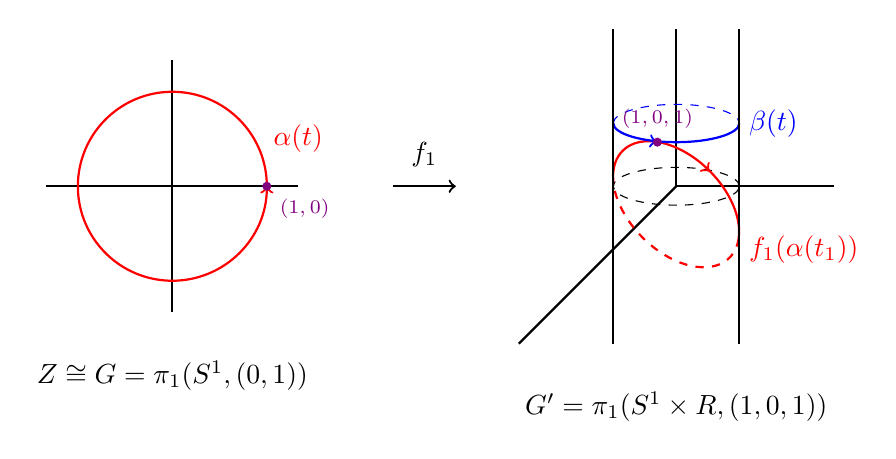
\begin{tikzpicture}[scale=0.8]
            \shorthandoff{>}

            \begin{scope}[shift={(-4,0)}]
                % Ejes
                \draw[thick] (-2,0) -- (2,0);
                \draw[thick] (0,-2) -- (0,2);

                % Circunferencia
                \draw[thick, red, ->] (1.5,0) arc (0:360:1.5 and 1.5);
                \node[red] at (2,0.75) {$\alpha(t)$};

                % Punto
                \node[draw, circle, fill=black,, violet, inner sep=1pt, label={[violet]below right:{\scriptsize $(1,0)$}}] at (1.5,0) {};


                % Leyenda
                \node at (0,-3) {$\bb{Z} \cong G = \pi_1(\bb{S}^1,(0,1))$};

            \end{scope}

            \node at (0,0.5) {$f_1$};
            \draw[thick,->] (-0.5,0) -- (0.5,0);

            \begin{scope}[shift={(4,0)}]
                % Ejes
                \draw[thick] (0,0) -- (0,2.5);
                \draw[thick] (0,0) -- (2.5,0);
                \draw[thick] (0,0) -- (-2.5,-2.5);
                \draw[dashed] (0,0) ellipse (1 and 0.3);

                % f_1(\alpha(t_1))
                \draw[red, thick, dashed, rotate around={-45:(0,-0.3)}] (1.075,0.025)  arc (25:-155:1.2 and 0.75);
                \draw[red, thick, rotate around={-45:(0,-0.3)}] (1.075,0.025)  arc (25:210:1.2 and 0.75);
                \draw[->, red, thick, rotate around={-45:(0,-0.3)}] (0,0.45) ++(-0.02, 0) -- ++(0.01,0);
                \node[red, anchor=west] at (1,-1) {$f_1(\alpha(t_1))$};
                
                % Beta
                \draw[dashed, blue] (-1,1) arc (180:0:1 and 0.3);
                \draw[thick, blue] (-1,1) arc (-180:0:1 and 0.3);
                \draw[->, blue, thick] (-0.3,0.7) ++(-0.02, 0.01) -- ++(0.01,-0.001);
                \node[blue, anchor=west] at (1,1) {$\beta(t)$};

                

                % Punto
                \node[draw, circle, fill=black,, violet, inner sep=1pt, label={[violet]above:{\scriptsize $(1,0,1)$}}] at (-0.3,0.7) {};

                % Cilindro 
                \draw[thick] (-1,-2.5) -- (-1,2.5);
                \draw[thick] (1,-2.5) -- (1,2.5);

                % Leyenda
                \node at (0,-3.5) {$G' = \pi_1(\bb{S}^1 \times \bb{R},(1,0,1))$};
            \end{scope}
        \end{tikzpicture}
    \end{figure}

    podemos ver que $\pi_1(\bb{S}^1,(1,0))$ está generado por $[\alpha]$ donde 
    \begin{gather*}
        \alpha(t) = (\cos(2\pi t), \sen(2\pi t))
    \end{gather*}
    y $\pi_1(\bb{S}^1\times \bb{R}, (1,0,1))$ está generado por $[\beta]$ donde 
    \begin{gather*}
        \beta(t) = (\cos(2\pi t), \sen(2\pi t), 1)
    \end{gather*}
    Además es fácil ver en la misma gráfica que
    \begin{gather*}
        f_{1*}([\alpha]) = [f_1 \circ \alpha] = [\beta]\\
        f_{1*}(\pi_1(\bb{S}^1, (1,0))) = \pi_1(\bb{S}^1\times \bb{R}, (1,0,1))
    \end{gather*}
    Ahora calculamos
    \begin{gather*}
        p_*(\pi_1(\bb{S}^1 \times \bb{R}, (1,0,1)))
    \end{gather*}
    Sabemos que 
    \begin{gather*}
        \pi_1(\bb{S}^1 \times \bb{R}, (1,0,1)) = \{[\beta]^n : n\in \bb{Z}\}
    \end{gather*}
    y además
    \begin{align*}
        (p\circ \beta)(t) &= (\cos^2(2\pi t) - \sen^2(2\pi t), 2\cos (2\pi t)\sen(2\pi t), 1) =\\
        &= (\cos(4\pi t), \sen(4\pi t), 1) = (\beta \ast \beta)(t)
    \end{align*}
    por lo que 
    \begin{gather*}
        p_*([\beta]) = [p\circ \beta] = [\beta]^2\\
        p_*(\pi_1(\bb{S}^1 \times \bb{R}, (1,0,1))) = \{[\beta]^{2n} : n\in \bb{Z}\}
    \end{gather*}

    Sabemos por el teorema visto que existe un $\hat{f_1} : \bb{S}^1 \to \bb{S}^1 \times \bb{R}$ levantamiento de $f_1$ con $\hat{f_1}(1,0)=(1,0,1)$ si y solo si se tiene que 
    \begin{gather*}
        f_{1*}(\pi_1(\bb{S}^1, (1,0))) \subseteq p_*(\pi_1(\bb{S}^1 \times \bb{R}, (1,0,1)))
    \end{gather*}
    Como tenemos que 
    \begin{gather*}
        f_{1*}(\pi_1(\bb{S}^1, (1,0))) = \{[\beta]^k : k\in \bb{Z}\} \cong \bb{Z} \\
        p_*(\pi_1(\bb{S}^1 \times \bb{R}, (1,0,1))) = \{[\beta]^{2m}: m\in \bb{Z}\} \cong 2\bb{Z}
    \end{gather*}
    no se dará la inclusión 
    \begin{gather*}
        f_{1*}(\pi_1(\bb{S}^1, (1,0))) \nsubseteq p_*(\pi_1(\bb{S}^1 \times \bb{R}, (1,0,1)))
    \end{gather*}
    y tenemos que no existe $\hat{f_1} : \bb{S}^1 \to \bb{S}^1 \times \bb{R}$ levantamiento de $f_1$ con $\hat{f_1}(1,0)=(1,0,1)$.

    Si tomamos otro punto $r_1$ cualquiera tal que $p(r_1)=(1,0,1)$ ($r_1$ solo podría ser el $(-1,0,1)$) entonces sabemos por un corolario anterior que 
    \begin{gather*}
        p_*(\pi_1(\bb{S}^1\times \bb{R}, r_1)) \text{ es conjugado de } p_*(\pi_1(\bb{S}^1 \times \bb{R}, (1,0,1)))
    \end{gather*}
    Como el grupo total es abeliano, entonces estos dos grupos son idénticos.\\
    
    Veamos qué ocurre con $f_2$. En este caso tenemos que 
    \begin{gather*}
        f_2(1,0) = (0,1,1)
    \end{gather*}
    Además, $[\alpha]$ genera $\pi_1(\bb{S}^1, (1,0))$ y $[\gamma]$ genera $\pi_1(\bb{S}^1 \times \bb{R}, (0,1,1))$ donde 
    \begin{gather*}
        \gamma(t) = \left(\cos\left(2\pi t + \frac{\pi}{2}\right), \sen\left(2\pi t + \frac{\pi}{2}\right), 1\right)
    \end{gather*}
    Queremos calcular $f_2\circ \alpha$:
    \begin{align*}
        (f_2\circ \alpha)(t) &= (-2\cos(2\pi t)\sen(2\pi t), \cos^2(2\pi t) - \sen^2(2\pi t), \cos^2(2\pi t)) = \\
        &= (-\sen(4\pi t), -\cos(4\pi t), \cos^2(2\pi t)) =\\
        &= (\sen(-4\pi t), \cos(-4\pi t), \cos^2(2\pi t)) =\\
        &= \left(\cos\left(\frac{\pi}{2} + 4\pi t\right), \sen\left(\frac{\pi}{2} + 4\pi t\right), \cos^2(2\pi t)\right)
    \end{align*}
    y podemos concluir que 
    \begin{gather*}
        f_{2*}([\alpha]) = [f_2\circ \alpha] = [\gamma \ast \gamma] = [\gamma]^2
    \end{gather*}
    por lo que
    \begin{align*}
        f_{2*}(\pi_1(\bb{S}^1,(1,0))) &= \{[\gamma]^{2n} : n\in \bb{Z}\} =\\
        &= p_*\left(\pi_1\left(\bb{S}^1 \times \bb{R}, \left(\frac{1}{\sqrt{2}}, \frac{1}{\sqrt{2}}, 1\right)\right) \right) 
    \end{align*}
    y tenemos finalmente que existe el levantamiento $\hat{f_2}$ con $\hat{f_2}(1,0)=(0,1,1)$
\end{ejemplo}

\section{Transformación de recubridores}

Vamos a tratar en lo que queda de tema de clasificar los espacios recubridores de un espacio topológico $B$ dado. Comenzamos estableciendo para ello una nomenclatura clásica.

\begin{notacion}
    Diremos que $(R,p)$ es un recubridor de $B$ si $p:R\to B$ es una aplicación recubridora.
\end{notacion}

\begin{definicion}
    Sean $(R_1,p_2)$, $(R_2,p_2)$ dos espacios recubridores de un mismo e.t. base $B$, 
    \begin{gather*}
        \xymatrix{
            R_1 \ar[dr]_{p_1} & & R_2 \ar[dl]^{p_2}\\
            & B
        }
    \end{gather*}
    \begin{enumerate}
        \item Un \textbf{homomorfismo de recubridores} $\phi$ de $(R_1,p_1)$ en $(R_2,p_2)$ es una aplicación continua $\phi:R_1 \to R_2$  tal que $p_2 \circ \phi = p_1$. Dicha aplicación hace que el siguiente diagrama conmute:
        \begin{gather*}
            \xymatrix{
                R_1 \ar[dr]_{f=p_1} \ar[rr]^{\hat{f}=\phi} & & R_2 \ar[dl]^{p_2}\\
                & B
            }
        \end{gather*}
        O equivalentemente $\phi$ es un levantamiento de la aplicación continua $p_1$ usando la aplicación recubridora $p_2$.

        \item Un \textbf{isomorfismo de recubridores} $\phi$ de $(R_1,p_1)$ es $(R_2,p_2)$ es un homeomorfismo $\phi:R_1 \to R_2$ tal que $p_2 \circ \phi = p_1$.

        \item Un isomorfismo $\phi$ de $(R_1,p_1)$ es sí mismo se le llama \textbf{automorfismo de recubridores}. Al conjunto de todos los automorfismos lo notaremos por $\cc{A}(R_1,p_1)$.
    \end{enumerate}
\end{definicion}

\begin{observacion}\
    \begin{enumerate}
        \item Si $(R,p)$ es un recubridor de un espacio base $B$ y $\phi:\hat{R}\to R$ es un homeomorfismo, entonces $(\hat{R}, p\circ \phi)$ es un recubridor de $B$. Se puede ver fácilmente con el siguiente diagrama:
        \begin{gather*}
            \xymatrix{
                \hat{R} \ar[r]^{\phi} \ar[dr]_{p\circ \phi} & R \ar[d]^{p}\\
                & B
            }
        \end{gather*}
        recordando que la composición de una aplicación recubridora con un homeomorfismo es también una aplicación recubridora (visto en las propiedades de las aplicaciones recubridoras). Además, $\phi$ de $(\hat{R}, p\circ \phi)$ en $(R,p)$ es un isomorfismo de recubridores. De hecho, de la definición se deduce que todo isomorfismo de recubridores es de la forma anterior.

        \item Si $\phi_1$ de $(R_1,p_1)$ es $(R_2,p_2)$ es un homomorfismo de recubridores y $\phi_2$ es otro desde $(R_2,p_2)$ en $(R_3,p_3)$, entonces $\phi_2\circ \phi_1$ es un homomorfismo de recubridores de $(R_1,p_1)$ en $(R_3, p_3)$. Tendríamos la situación del siguiente diagrama:
        \begin{gather*}
            \xymatrix{
                R_1 \ar[dr]_{p_1} \ar[r]^{\phi_1} & R_2 \ar[d]^{p_2} \ar[r]^{\phi_2} & R_3 \ar[dl]^{p_3}\\
                & B 
            }
        \end{gather*}

        \item Si $\phi$ es un isomorfismo de recubridores desde $(R_1,p_1)$ en $(R_2,p_2)$, entonces $\phi^{-1}$ es un isomorfismo de recubridores desde $(R_2,p_2)$ en $(R_1,p_1)$.
        \begin{gather*}
            \xymatrix{
                R_1 \ar@/_/[rr]_{\phi} \ar[dr]_{p_2} && R_2 \ar@/_/[ll]_{\phi^{-1}} \ar[dl]^{p_2} \\
                & B
            }
        \end{gather*}

        \item $\cc{A}(R,p)$ es un grupo con la composición.
    \end{enumerate}
\end{observacion}

\begin{coro}\label{coro-2.3.1}
    Sean $\phi_1$, $\phi_2$ dos homomorfismos de recubridores desde $(R_1,p_1)$ en $(R_2,p_2)$. Entonces se tiene que 
    \begin{gather*}
        \phi_1 = \phi_2 \sii \exists r_1\in R_1 : \phi_1(r_1) = \phi_2(r_1)
    \end{gather*}
    En particular, si $\phi$ es un homomorfismo de un recubridor $(R,p)$ en sí mismo, entonces
    \begin{gather*}
        \phi = Id_{R} \sii \exists r \in R : \phi(r)=r
    \end{gather*}

    \begin{proof}
        Estamos en la siguiente situación
        \begin{gather*}
            \xymatrix{
                R_1 \ar@/^/[rr]^{\phi_2} \ar@/_/[rr]_{\phi_1} \ar[dr]_{p_1} && R_2 \ar[dl]^{p_2} \\
                & B
            }
        \end{gather*}

        Veamos la doble implicación de la primera mitad del corolario
        \begin{itemize}
            \item[$\Rightarrow$)] Es trivial que si $\phi_1=\phi_2$ entonces $\forall r \in R_1$ se tiene que $\phi_1(r)=\phi_2(r)$.
            \item[$\Leftarrow$)] Supongamos que $\exists r_1\in R_1$ tal que $\phi_1(r_1)=\phi_2(r_1)$. Entonces, como $\phi_1$ y $\phi_2$ son levantamientos de $p_1$, por el teorema de unicidad del levantamiento tenemos que $\phi_1=\phi_2$.
        \end{itemize}

        Para probar la segunda parte del corolario aplicaremos lo ya probado tomando $\phi_1=\phi$ un homomorfismo de un recubridor $(R,p)$ en sí mismo y $\phi_2=Id_R$.
        \begin{gather*}
            \xymatrix{
                R \ar@/^/[rr]^{Id_R} \ar@/_/[rr]_{\phi} \ar[dr]_{p} && R \ar[dl]^{p} \\
                & B
            }
        \end{gather*}
        Entonces tendríamos que 
        \begin{gather*}
            \phi = Id_R \sii \exists r\in R : \phi(r)=Id_R(r)=r
        \end{gather*}
    \end{proof}
\end{coro}

\begin{coro}
    Sean $(R_1,p_1)$, $(R_2, p_2)$ dos recubridores de $B$, $b_0\in B$ y $r_1\in p_{1}^{-1}(b_0)$, $r_2\in p_2^{-1}(b_0)$. Entonces:
    \begin{enumerate}
        \item Existe un homomorfismo de recubridores $\phi$ de $(R_1,p_1)$ en $(R_2, p_2)$ con $\phi(r_1)=r_2$ si y solo si 
        \begin{gather*}
            p_{1*}(\pi_1(R_1,r_1)) \subseteq p_{2*}(\pi_1(R_2,r_2))
        \end{gather*}

        \item Existe un isomorfismo de recubridores $\phi$ de $(R_1,p_1)$ en $(R_2, p_2)$ con $\phi(r_1)=r_2$ si y solo si
        \begin{gather*}
            p_{1*}(\pi_1(R_1,r_1)) = p_{2*}(\pi_1(R_2,r_2))
        \end{gather*}
    \end{enumerate}

    \begin{proof}
        Veamos cada punto por separado.
        \begin{enumerate}
            \item Estamos en la siguiente situación (donde se ha puesto la equivalencia con la notación que usamos para el teorema de existencia del levantamiento)
            \begin{gather*}
                \xymatrix{
                    X = R_1 \ar[rr]^{\phi \overset{?}{\equiv} \hat{f}} \ar[dr]_{f=p_1} && R_2=R \ar[dl]^{p_2=p} \\
                    & B
                }
            \end{gather*}
            Entonces por el teorema de existencia del levantamiento tenemos que existe $\phi$ levantamiento de $p_1$ con $\phi(r_1) = r_2$ si y solo si 
            \begin{gather*}
                p_{1*}(\pi_1(R_1,r_1)) \subseteq p_{2*}(\pi_1(R_2,r_2))
            \end{gather*}

            \item Veamos la doble implicación. 
            \begin{itemize}
                \item[$\Rightarrow$)] Queremos ver que se verifica la igualdad entre las imágenes de los homomorfismos inducidos de los grupos fundamentales. Veámoslo por doble inclusión. En primer lugar denotamos por $\phi$ al isomorfismo y a su inversa la llamaremos $\varphi$. Esta aplicación verifica  que
                \begin{gather*}
                    \varphi \circ \phi = Id_{R_1} \ \ \ \ \phi \circ \varphi = Id_{R_2}
                \end{gather*}
                y además es también un isomorfismo (por lo que en particular es un homomorfismo). Estaríamos en la situación del siguiente diagrama
                \begin{gather*}
                    \xymatrix{
                        R_1 \ar[r]^{\phi} \ar[dr]_{p_1} & R_2 \ar[d]^{p_2} \ar[r]^{\varphi} & R_1\ar[dl]^{p^1} \\
                        & B
                    }
                \end{gather*}
                donde $\phi$ y $\varphi$ son homomorfismos. Por hipótesis tenemos que $\exists r_1\in p_1^{-1}(b_0)$, $r_2\in p_2^{-1}(b_0)$ tales que $\phi(r_1)=r_2$. Si componemos esta igualdad por la izquierda con $\varphi$ tenemos
                \begin{gather*}
                    (\varphi \circ \phi) (r_1) = \varphi(r_2) \Rightarrow Id_R(r_1) = \phi(r_2) \Rightarrow r_1 = \varphi(r_2)
                \end{gather*}
                Por tanto aplicando el primer punto del corolario a $\phi$ (es un homomorfismo con $\phi(r_1)=r_2$) tenemos que 
                \begin{gather*}
                    p_{1*}(\pi_1(R_1,r_1)) \subseteq p_{2*}(\pi_1(R_2,r_2))
                \end{gather*}
                y aplicando lo mismo de nuevo a $\varphi$ (es un homomorfismo con $\varphi(r_2)=r_1$) tenemos que 
                \begin{gather*}
                    p_{2*}(\pi_2(R_2,r_2)) \subseteq p_{1*}(\pi_1(R_1,r_1))
                \end{gather*}
                por lo que llegamos finalmente a que 
                \begin{gather*}
                    p_{1*}(\pi_1(R_1,r_1)) = p_{2*}(\pi_1(R_2,r_2))
                \end{gather*}

                \item[$\Leftarrow$)] Supongamos que $p_{1*}(\pi_1(R_1,r_1)) = p_{2*}(\pi_1(R_2,r_2))$. Buscamos aplicar ahora el punto anterior a este caso. De la siguiente inclusión
                \begin{gather*}
                    p_{1*}(\pi_1(R_1,r_1)) \subseteq p_{2*}(\pi_1(R_2,r_2))
                \end{gather*}
                tenemos que existe un homomorfismo de recubridores $\phi$ de $(R_1,p_1)$ en $(R_2,p_2)$ con $\phi(r_1)=r_2$. Análogamente, de la siguiente inclusión  
                \begin{gather*}
                    p_{2*}(\pi_1(R_2,r_2)) \subseteq p_{1*}(\pi_1(R_1,r_1))
                \end{gather*}
                tenemos que existe un homomorfismo de recubridores $\varphi$ de $(R_2,p_2)$ en $(R_1,p_1)$ con $\varphi(r_2)=r_1$. Podemos considerar entonces su composición $\varphi \circ \phi$, que es claramente un homomorfismo de $(R_1,p_1)$ en sí mismo con $\varphi(\phi(r_1)) = r_1$. Por el corolario \ref{coro-2.3.1} tenemos que 
                \begin{gather*}
                    \varphi \circ \phi = Id_{R_1}
                \end{gather*}
                Análogamente podemos llegar a que
                \begin{gather*}
                    \phi \circ \varphi = Id_{R_2}
                \end{gather*}
                Tenemos entonces que $\phi$ es una aplicación continua, $\varphi$ es su inversa y además es también continua, luego $\phi$ es un homeomorfismo. Este será el que nos dé el isomorfismo de recubridores de $(R_1, p_1)$ en $(R_2, p_2)$.
            \end{itemize}

        \end{enumerate}
    \end{proof}
\end{coro}

\begin{teo}
    Sean $(R_1, p_1)$, $(R_2, p_2)$ dos recubridores de un e.t. $B$. Entonces existe un isomorfismo entre ambos recubridores si y solo si dado $b_0\in B$ existen $r_1\in R_1$ y $r_2 \in R_2$ con $p_1(r_1) = b_0 = p_2(r_2)$ tales que 
    \begin{gather*}
        p_{1*}(\pi_1(R_1,r_1)) = p_{2*}(\pi_1(R_2,r_2))
    \end{gather*}
    \begin{proof}
        Estamos en la siguiente situación
        \begin{gather*}
            \xymatrix{
                R_1 \ar[dr]_{p_1} && R_2 \ar[dl]^{p_2}\\
                & B
            }
        \end{gather*}
        Veamos la doble implicación
        \begin{itemize}
            \item[$\Rightarrow$)] Supongamos primero que existe $\phi$ isomorfismo de recubridores de $(R_1, p_1)$ en $(R_2, p_2)$. Tomamos $b_0\in B$ y elegimos $r_1\in p_1^{-1}(b_0)$ cualquiera (que existe porque $p_1$ e sobreyectiva). Elegimos $r_2 = \phi(r_1)$ y entonces como $p_2\circ \phi = p_1$ tenemos que 
            \begin{align*}
                p_{1*}(\pi_1(R_1,r_1)) &= (p_2\circ \phi)_*(\pi_1(R_1, r_1)) = \\
                &= p_{2*}(\phi_*(\pi_1(R_1,r_1))) = p_{2*}(\pi_1(R_2, r_2))
            \end{align*}
            ya que como $\phi$ es un homomorfismo tenemos que $\phi_*(\pi_1(R_1,r_1)) = \pi_1(R_2, \phi(r_1))$.

            \item[$\Leftarrow$)] Está probada aplicando el corolario anterior.
        \end{itemize}
    \end{proof}
\end{teo}

\begin{observacion}
    Algunas consecuencias que podemos extraer de lo anterior son las siguientes:\\

    Sean $B$ un e.t. y $b_0\in B$. Si consideramos $H$ un subgrupo de $\pi_1(B,b_0)$ entonces
    \begin{enumerate}
        \item Existe como mucho un recubridor $(R,p)$ (salvo isomorfismo) cumpliendo que $\exists r\in R$ tal que $p_*(\pi_1(R,r)) = H$.
        \begin{gather*}
            \xymatrix{
                R \ar[d]_p & \pi_1(R,r)\ar[d]_{p_*}\\
                B & H \leq \pi_1(B,b_0)
            }
        \end{gather*}
        
        \item Además si $H$ y $H'$ son subgrupos conjugados en $\pi_1(B,b_0)$, como mucho existe un recubridor correspondiente a ambos, es decir, si $(R,p)$ es un recubridor con $r_0\in R$ tal que $p_*(\pi_1(R,r_0)) = H$, entonces también existe un $r_0'\in R$ tal que $p_*(\pi_1(R,r_0'))=H'$.
        \begin{gather*}
            \xymatrix{
                R \ar[d]_p & \pi_1(R,r)\ar[d]_{p_*} & \pi_1(R,r') \ar[d]_{p_*}\\
                B & H \leq \pi_1(B,b_0) & H'\leq \pi_1(B,b_0)
            }
        \end{gather*}
    \end{enumerate}
\end{observacion}

\begin{ejemplo}\
    \begin{enumerate}
        \item Consideramos $B=\bb{R}$ y buscamos los recubridores de $\bb{R}$. Tenemos que 
        \begin{gather*}
            \pi_1(\bb{R},0) = \{[\veps_0]\}
        \end{gather*}
        Por lo que solo hay un subgrupo $H=\{[\veps_0]\}$, luego $\bb{R}$ solo tiene un recubridor
        \begin{gather*}
            (\bb{R}, p= Id_{\bb{R}})
        \end{gather*}

        \item En general, si $B$ es simplemente conexo, entonces su único recubridor es él mismo (salvo isomorfismo de recubridores).
        
        \item Consideramos ahora $\bb{R}\bb{P}^n$ el espacio proyectivo con $n\geq 2$. Tenemos que
        \begin{gather*}
            \pi_1(\bb{R}\bb{P}^n, x_0) \cong \bb{Z}_2, \text{ con } x_0\in \bb{R}\bb{P}^n \text{ cualquiera}
        \end{gather*}
        Por tanto tendríamos que los únicos posibles subgrupos de $\pi_1(\bb{R}\bb{P}^n, x_0)$ son
        \begin{gather*}
            H_1 = \{[\veps_{x_0}]\} \to \text{ Recubridor asociado } (\bb{S}^n, p) \text{ con } p(x)=[x]\\
            H_2 \cong \bb{Z}_2 \to \text{ Recubridor asociado } (\bb{R}\bb{P}^n, Id_{\bb{R}\bb{P}^n})
        \end{gather*}
        \begin{gather*}
            \xymatrix{
                R \ar[d]_p & r_0 \ar@{|->}[d] & \{0\} \ar@{|->}[d] & \bb{R}\bb{P}^n \ar[d]_{Id} & x_0 \ar@{|->}[d]_{Id} & \pi_1(\bb{R}\bb{P}^n, x_0) \ar[d]^{Id_*}\\
                \bb{R}\bb{P}^n & x_0  & \{0\} & \bb{R}\bb{P}^n & x_0 & \pi_1(\bb{R}\bb{P}^n, x_0)
            }
        \end{gather*}
        por lo que los únicos recubridores de $\bb{R}\bb{P}^2$ son $(\bb{S}^n, p)$ con $p(x)=[x]$ y $(\bb{R}\bb{P}^n, Id_{\bb{R}\bb{P}^n})$.

        \item Consideramos $B=\bb{S}^1$. Recordemos que 
        \begin{gather*}
            \pi_1(\bb{S}^1, (1,0)) = \{[\alpha]^n : \alpha(t) = (\cos(2\pi t), \sen(2\pi t)),\ n\in \bb{Z}\} \cong \bb{Z}
        \end{gather*}
        Los únicos subgrupos de $\bb{Z}$ son 
        \begin{gather*}
            H_k \cong k\bb{Z} \text{ donde } H_k = \{[\alpha]^{nk} : n\in \bb{Z}\} \text{ con } k\in \bb{Z}^+\\
            H_0 \cong \{0\}
        \end{gather*}

        Recordamos el recubrimiento de $\bb{S}^1$ que estudiamos en el tema anterior:

        \begin{figure}[H]
            \centering
            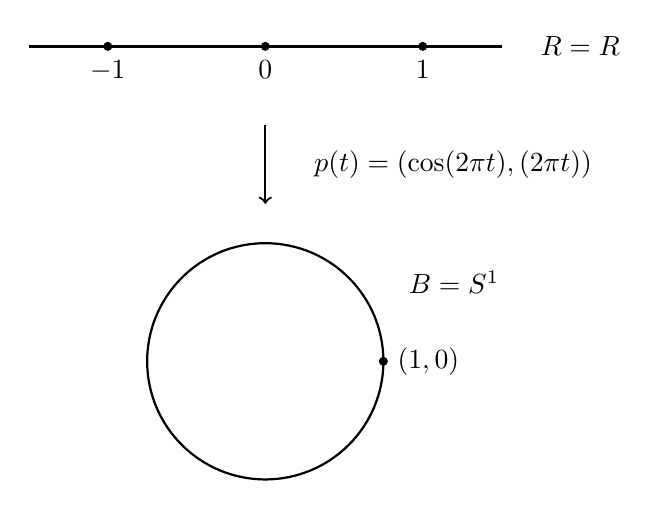
\begin{tikzpicture}{scale=0.7}
                \shorthandoff{>}
                % Recta
                \draw[line width=1pt] (-3,3) -- (3,3);
                \node at (4,3) {$R = \bb{R}$};

                % Puntos
                \node[draw, circle, fill=black, inner sep=1pt, label=below:$-1$] at (-2,3) {};
                \node[draw, circle, fill=black, inner sep=1pt, label=below:$0$] at (0,3) {};
                \node[draw, circle, fill=black, inner sep=1pt, label=below:$1$] at (2,3) {};

                % Flecha función
                \draw[line width=0.8pt,->] (0,2) -- (0,1);
                \node[anchor=west] at (0.5,1.5) {$p(t) = (\cos(2\pi t), \sen(2\pi t))$};

                % Circunferencia
                \draw[thick] (0,-1) circle [radius=1.5];
                \node[anchor=west] at (1.7,0) {$B=\bb{S}^1$};
                \node[draw, circle, fill=black, inner sep=1pt, label=right:{$(1,0)$}] at (1.5,-1) {};

            \end{tikzpicture}%
        \end{figure}%
        Para este recubridor $(\bb{R}, p)$ donde $p(t) = (\cos(2\pi t), \sen(2\pi t))$, su subgrupo asociado en $\pi_1(\bb{S}^1, (1,0))$ es $H_0$. Para ver que efectivamente es $H_0$ podemos considerar el generador de $\pi_1(\bb{R}, 0)$ que, por ser $\bb{R}$ simplemente conexo será un lazo trivial $[\veps_0]$. Si estudiamos la imagen de este generador tendremos 
        \begin{gather*}
            (p\circ \veps_0)(t) = p(\veps_0(t)) = p(0) = (1,0)
        \end{gather*}
        por lo que $p_*(\pi_1(\bb{R},0)) = \{[\veps_{(1,0)}]\} \cong \{0\}\cong H_0$.\\

        También podemos considerar el recubridor $(\bb{S}^1, p_1=Id_{\bb{S}^1})$ cuyo subgrupo asociado es $H_1 = \pi_1(\bb{S}^1, (1,0))$.\\

        Ahora nos planteamos de nuevo que $\bb{S}^1$ es recubridor de sí mismo pero que hay más formas de recubrirse, es decir, podemos encontrar funciones recubridoras $p_k$ con $k\in \bb{Z}^+$ de forma que todas recubran a la circunferencia pero ``enrollandola más'', es decir, llevando cada vuelta de $R=\bb{S}^1$ en $k$ vueltas de $B=\bb{S}^1$. Definimos así la aplicación $p_k$ para $k\geq 2$ (el caso $k=1$ es la identidad que ya se ha estudiado) dada por 
        \Func{p_k}{\bb{S}^1}{\bb{S}^1}
             {(\cos(\theta), \sen(\theta))}{(\cos(k\theta), \sen(k\theta))}
        Además tendríamos que 
        \Func{ p_{k*}}{\pi_1(\bb{S}^1, (1,0))}{\pi_1(\bb{S}^1, (1,0))}
             {[\alpha]}{[\alpha]^k}
        Llegando a que 
        \begin{gather*}
            p_{k*}(\pi_1(\bb{S}^1, (1,0))) = H_k = \{[\alpha]^{kn} : n\in \bb{Z}\}
        \end{gather*}
        Por tanto, los únicos recubridores de $\bb{S}^1$ son
        \begin{gather*}
            (\bb{R}, p)\text{ con } p(t)=(\cos(2\pi t), \sen(2\pi t))\\
            (\bb{S}^1, p_k)\text{ con } p_k(\cos(\theta), \sen(\theta)) = (\cos(k\theta), \sen(k\theta)) \text{ para todo } k\in \bb{Z}^+
        \end{gather*}

        \item Vamos a estudiar ahora los recubridores del cilindro de $\bb{R}^3$, $B=\bb{S}^1\times \bb{R}$. Sabemos que
        \begin{gather*}
            \pi_1(\bb{S}^1\times \bb{R}, (1,0,0)) = \{[\alpha]^n : n\in \bb{Z}\} \cong \bb{Z}
        \end{gather*}
        por lo que tenemos de nuevo que los únicos subgrupos de $\bb{Z}$ son 
        \begin{gather*}
            H_k \cong k\bb{Z} \text{ donde } H_k = \{[\alpha]^{nk} : n\in \bb{Z}\} \text{ con } k\in \bb{Z}^+\\
            H_0 \cong \{0\}
        \end{gather*}
        y además sabemos que $(\bb{R}^2, p_0)$ es recubridor del cilindro con
        \Func{p_0}{\bb{R}^2}{\bb{S}^1\times \bb{R}}
             {(x,y)}{(\cos(2\pi x), \sen(2\pi x), y)}
        asociado a $H_0=\{[\veps_{(1,0,0)}]\}$.\\

        Buscamos ahora los recubridores cuyo subgrupo asociado es $H_k$.  Con la misma idea que en el ejemplo anterior definimos la función $p_k$ para $k\in \bb{Z}^+$ dada por 
        \Func{p_k}{\bb{S}^1 \times \bb{R}}{\bb{S}^1 \times \bb{R}}
             {(\cos(\theta), \sen(\theta), y)}{(\cos(k\theta), \sen(k\theta), y)}
        Al igual que en el ejemplo anterior tenemos que 
        \begin{gather*}
            p_{k*}([\alpha]) = [\alpha]^k\\
            p_{k*}(\pi_1(\bb{S}^1 \times \bb{R}, (1,0,0))) = \{[\alpha]^{kn} : n\in \bb{Z}\} = H_k
        \end{gather*}
        Por tanto los únicos recubridores del cilindro $\bb{S}^1\times \bb{R}$ son 
        \begin{gather*}
            (\bb{R}^2, p_0) \text{ con } p_0(x,y) = (\cos(2\pi x), \sen(2\pi x), y)\\
            (\bb{S}^1\times \bb{R}, p_k) \text{ con } p_k(\cos(\theta), \sen(\theta), y) = (\cos(k\theta), \sen(k\theta), y) \text{ para todo } k\in \bb{Z}^+
        \end{gather*}

        \item Veamos el caso del toro, $B=\bb{S}^1 \times \bb{S}^1$. Sabemos que 
        \begin{gather*}
            \pi_1(\bb{S}^1\times \bb{S}^1, (1,0,1,0)) \cong \bb{Z}\times \bb{Z}
        \end{gather*}
        con generadores $[\alpha]$ y $[\beta]$.\\

        Consideramos el recubridor $(\bb{R}^2, p_0\times p_0)$ con 
        \Func{p_0\times p_0}{\bb{R}^2}{\bb{S}^1 \times \bb{S}^1}
             {(x,y)}{(cos(2\pi x), \sen(2\pi x), \cos(2\pi y), \sen(2\pi y))}
        Como $\pi_1(\bb{R}^2, (0,0)) = [\veps_{(0,0)}]$ tenemos que 
        \begin{gather*}
            (p_0\times p_0)_*(\pi_1(\bb{R}^2, (0,0))) = \{[\veps_{(1,0,1,0)}]\}
        \end{gather*}
        por lo que $(\bb{R}^2, p_0\times p_0)$ es el recubridor asociado al subgrupo trivial de $\pi_1(\bb{S}^1\times \bb{S}^1, (1,0,1,0))$.\\

        Consideramos ahora el cilindro como recubridor y definimos la aplicación recubridora
        \Func{p_k\times p_0}{\bb{S}^1\times \bb{R}}{\bb{S}^1 \times \bb{S}^1}
             {(\cos(\theta), \sen(\theta), y)}{(cos(k\theta), \sen(k\theta), \cos(2\pi y), \sen(2\pi y))}
        que para cada $k\in \bb{Z}^+$ ``enrolla'' el cilindro $k$ veces. 
        En este caso tendríamos que 
        \begin{gather*}
            (p_k\times p_0)(1,0,0) = (1,0,1,0)
        \end{gather*}
        y además tenemos que 
        \begin{gather*}
            \pi_1(\bb{S}^1 \times \bb{R}, (1,0,0)) = \{[\gamma]^n : n\in \bb{Z}\} \text{ donde } \gamma(t)=(\cos(2\pi t), \sen(2\pi t), 0)
        \end{gather*}
        Tenemos además que $(p_k\times p_0)(\gamma(t)) = (\cos(2k\pi t), \sen(2k\pi t), 1, 0)$ de donde se deduce que
        \begin{gather*}
            (p_k \times p_0)_*([\gamma]) = [(p_k\times p_0)(\gamma)]
            = [\alpha]^k 
        \end{gather*}
        Una vez hemos calculado la imagen del generador podemos concluir que 
        \begin{gather*}
            (p_k\times p_0)_*(\pi_1(\bb{S}^1 \times \bb{R}, (1,0,0))) = \{[\alpha]^{nk} : n\in \bb{Z}\} \cong k\bb{Z}\times \{0\} \leq \bb{Z} \times \bb{Z}
        \end{gather*}
        Análogamente si consideramos 
        \Func{p_0\times p_k}{\bb{R}\times \bb{S}^1}{\bb{S}^1 \times \bb{S}^1}
             {(x,  \cos(\theta), \sen(\theta))}{(\cos(2\pi x), \sen(2\pi x), cos(k\theta), \sen(k\theta))}
        tendríamos el siguiente recubridor
        \begin{gather*}
            (\bb{R}\times \bb{S}^1, p_0\times p_k) \text{ asociado a } \{0\}\times k\bb{Z} \leq \bb{Z}\times \bb{Z}
        \end{gather*}
        Consideramos ahora el toro como recubridor de sí mismo y definimos
        \Func{p_k\times p_l}{\bb{S}^1\times \bb{S}^1}{\bb{S}^1 \times \bb{S}^1}
             {(\cos(\theta), \sen(\theta), \cos(\varphi), \sen(\varphi))}{(cos(k\theta), \sen(k\theta), \cos(l \varphi), \sen(l\varphi))}
        Si estudiamos la imagen de los generadores tenemos 
        \begin{gather*}
            (p_k\times p_l)_*([\alpha]) = [\alpha]^k\\
            (p_k\times p_l)_*([\beta]) = [\beta]^l
        \end{gather*}
        y llegamos a que $(\bb{S}^1 \times \bb{S}^1, p_k\times p_l)$ es recubridor y está asociado al subgrupo $k\bb{Z}\times l\bb{Z}$. El grupo imagen sería
        \begin{gather*}
            \{[\alpha]^{kn_1}\ast [\beta]^{ln_2} : n_1,n_2\in \bb{Z}\}
        \end{gather*}
        En este punto nos damos cuenta de que aún no hemos estudiado todos los subgrupos de $\bb{Z}\times \bb{Z}$. Si consideramos 2 puntos de $\bb{Z}$ podemos generar un subgrupo a partir de ellos, por ejemplo, para $(1,3), (2,4)\in \bb{Z}\times \bb{Z}$ podemos construir $\{a(1,3)+b(2,4) : a,b\in \bb{Z}\}$ y es un subgrupo de $\bb{Z}\times \bb{Z}$. Esto también ocurre con un solo generador. Es decir, tenemos que los subgrupos de $\bb{Z}\times \bb{Z}$ que nos queda por considerar son de la forma
        \begin{gather*}
            \{n(a,b) : n\in \bb{Z}\} \text{ para cada } (a,b)\in \bb{Z}\times \bb{Z}\\
            \{n_1(a,b) + n_2(c,d) : n_1,n_2\in \bb{Z}\} \text{ para cada } (a,b), (c,d)\in \bb{Z}\times \bb{Z}
        \end{gather*}
        Pensamos ahora entonces en la siguiente aplicación
        \Func{p'}{\bb{S}^1\times \bb{R}}{\bb{S}^1\times \bb{S}^1}
        {(cos(\theta), \sen(\theta), y)}{(\cos(\theta), \sen(\theta), \cos(\theta+y), \sen(\theta+y))}
        y nos planteamos quién sería $p'_*([\gamma])$. Aplicamos $p'$ en un generador y tenemos
        \begin{gather*}
            p'(\gamma(t)) = p(\cos(2\pi t), \sen(2\pi t), 0) = (\cos(2\pi t), \sen(2\pi t), \cos(2\pi t), \sen(2\pi t))
        \end{gather*}
        Intuitivamente podemos llegar a ver que $p'_*([\gamma]) = [\alpha] \ast [\beta]$.
        Esto se ha hecho considerando de fondo el generador $(1,1)$. Buscamos generalizar esta nueva aplicación recubridora para cualquier generador $(a,b)\in \bb{Z}\times \bb{Z}$. Se puede construir una aplicación $p'_{(a,b)}$ para cada $(a,b)\in \bb{Z}\times \bb{Z}$ de la siguiente forma:
        \Func{p'_{(a,b)}}{\bb{S}^1 \times \bb{R}}{\bb{S}^1\times \bb{S}^1}
        {(cos(\theta), \sen(\theta), y)}{(\cos(a\theta), \sen(a\theta), \cos(b\theta+y), \sen(b\theta+y))}
        Aplicando $p'_{(a,b)}$ en el generador tenemos
        \begin{gather*}
            p'_{(a,b)}(\gamma(t)) = p'(\cos(2\pi t), \sen(2\pi t), 0) = (\cos(2a\pi t), \sen(2a\pi t), \cos(2b\pi t), \sen(2b\pi t))
        \end{gather*}

        y con mucha intuición se puede llegar a que 
        \begin{gather*}
            (p'_{(a,b)})_*([\gamma]) = [\alpha]^a \ast [\beta]^b
        \end{gather*}

        Por tanto tenemos que $(\bb{S}^1 \times \bb{R}, p'_{(a,b)})$ es recubridor del toro con subgrupo asociado $\{n(a,b) : n\in \bb{Z}\}$ para cada generador que tomemos $(a,b)\in \bb{Z}$.\\

        De hecho, si tomamos un par de generadores $(a,b), (c,d)\in \bb{Z}\times \bb{Z}$ podemos definir la aplicación $p'_{(a,b)}\times p'_{(c,d)}: \bb{S}^1 \times \bb{S}^1 \to \bb{S}^1 \times \bb{S}^1$ dada por 
        \begin{gather*}
            (p'_{(a,b)}\times p'_{(c,d)})(\cos(\theta), \sen(\theta), \cos(\varphi), \sen(\varphi)) =\\
            = (\cos(a\theta + c\varphi), \sen(a\theta + c\varphi), \cos(b\theta + d\varphi), \sen(b\theta + d\varphi))
        \end{gather*}
        De esta forma, aplicando $p'_{(a,b)}\times p'_{(c,d)}$ en los generadores tenemos
        \begin{align*}
            (p'_{(a,b)}\times p'_{(c,d)})(\alpha(t)) &= (p'_{(a,b)}\times p'_{(c,d)})(\cos(2\pi t), \sen(2\pi t), 1, 0) =\\
            &= (p'_{(a,b)}\times p'_{(c,d)})(\cos(2\pi t), \sen(2\pi t), \cos(0), \sen(0)) =\\
            &= (\cos(2a\pi t), \sen(2a\pi t), \cos(2b\pi t), \sen(2b\pi t))\\\\
            (p'_{(a,b)}\times p'_{(c,d)})(\beta(t)) &= (p'_{(a,b)}\times p'_{(c,d)})(1, 0, \cos(2\pi t), \sen(2\pi t)) =\\
            &= (p'_{(a,b)}\times p'_{(c,d)})(\cos(0), \sen(0), \cos(2\pi t), \sen(2\pi t)) =\\
            &= (\cos(2c\pi t), \sen(2c\pi t), \cos(2d\pi t), \sen(2d\pi t))
        \end{align*}
        Por lo que de nuevo usando mucho la intuición (habría que demostrarlo formalmente) llegamos a que
        \begin{gather*}
            (p'_{(a,b)}\times p'_{(c,d)})_*([\alpha]) = [\alpha]^a \ast [\beta]^b\\
            (p'_{(a,b)}\times p'_{(c,d)})_*([\beta]) = [\alpha]^c \ast [\beta]^d
        \end{gather*}
        y tenemos que $(\bb{S}^1 \times \bb{S}^1, p'_{(a,b)}\times p'_{(c,d)})$ es recubridor del toro asociado al subgrupo $\{n_1(a,b) + n_2(c,d) : n_1,n_2\in \bb{Z}\}$ para cada par de generadores $(a,b),(c,d)\in \bb{Z}\times \bb{Z}$.\\

        Resumiendo, tenemos que todos los recubridores del toro $\bb{S}^1\times \bb{S}^1$ son 
        \begin{gather*}
            (\bb{R}^2, p_0\times p_0) \text{ asociado a } \{0\}\\
            (\bb{S}^1\times \bb{R}, p_k\times p_0) \text{ asociado a }k\bb{Z} \times \{0\} \text{ para cada } k\in \bb{Z}\\
            (\bb{R}\times \bb{S}^1, p_0\times p_k) \text{ asociado a } \{0\}\times k\bb{Z} \text{ para cada } k\in \bb{Z}\\
            (\bb{S}^1 \times \bb{S}^1, p_k\times p_l) \text{ asociado a } k\bb{Z}\times l\bb{Z} \text{ para cada } k,l\in \bb{Z}\\
            (\bb{S}^1\times \bb{R}, p'_{(a,b)}) \text{ asociado a } \{n(a,b) : n\in \bb{Z}\} \text{ para cada } (a,b)\in \bb{Z}\times \bb{Z}\\
            (\bb{S}^1\times \bb{R}, p'_{(a,b)}\times p'_{(c,d)}) \text{ asociado a } \{n_1(a,b) + n_2(c,d) : n_1,n_2\in \bb{Z}\}\\ \text{ para cada } (a,b),(c,d)\in \bb{Z}\times \bb{Z}
        \end{gather*}
        Como $\bb{Z}\times \bb{Z}$ no tiene más subgrupos estos serán todos los recubridores del toro.
    \end{enumerate}
\end{ejemplo}

Hasta ahora lo que hemos visto es que para estudiar el número de recubridores de un espacio $B$ podemos elegir un punto $b_0\in B$ y pasar a estudiar $\pi_1(B,b_0)$ y estudiando sus subgrupos $H<\pi_1(B,b_0)$ podíamos afirmar que como mucho había un recubridor por cada uno de ellos (o sus conjugados). Por tanto cuanto más ``grande'' sea el grupo fundamental, más recubridores podremos encontrar a priori. \\

\begin{prop}
    Sea $\phi$ un homomorfismo de recubridores desde $(R_1,p_1)$ en $(R_2,p_2)$. Entonces $\phi:R_1 \to R_2$ es una aplicación recubridora.
    \begin{gather*}
        \xymatrix{
            R_1 \ar[rr]^{\phi} \ar[dr]_{p_1} && R_2 \ar[dl]^{p_2}\\
            & B
        }
    \end{gather*}
    \begin{proof}
        Sabemos que $\phi$ es continua porque es homomorfismo. Veamos que $\phi$ es sobreyectiva (no es elemental). Consideramos un elemento cualquiera $r_2\in R_2$ y queremos ver si existe un $r_1\in R_1$ tal que $\phi(r_1)=r_2$. \\

        Tomamos $r_0\in R_1$ cualquiera y elegimos un arco $\alpha$ en $R_2$ que una $\phi(r_0)$ con $r_2$, es decir
        \begin{gather*}
            \alpha\in \Omega(R_2; \phi(r_0), r_2)
        \end{gather*}
        Si proyectamos tendremos que $p_2\circ \alpha$ es un arco en el espacio topológico base $B$ que une $p_2(\phi(r_2))$ con $p_2(r_2)$, es decir
        \begin{gather*}
            (p_2\circ \alpha) \in \Omega(B; p_2(\phi(r_0)), p_2(r_2))
        \end{gather*}
        Sabiendo que el diagrama de la proposición es conmutativo tenemos que $p_2(\phi(r_0)) = p_1(r_0)$. Como $p_1$ es aplicación recubridora, entonces tenemos que existe un único levantamiento $\widehat{p_2\circ \alpha}$ que comienza en $r_0$. Entonces tenemos que $\phi \circ \widehat{p_2\circ \alpha}$ es un arco en $R_2$ que comienza en $\phi(r_0)$. Es decir, $\alpha$ y $\phi\circ \widehat{p_2\circ \alpha}$ son dos arcos que empiezan en $\phi(r_0)$ y además
        \begin{gather*}
            p_2\circ(\phi \circ \widehat{p_2 \circ \alpha}) = p_1\circ(\widehat{p_2 \circ \alpha}) \overset{def}{=} p_2\circ \alpha
        \end{gather*}
        Por unicidad del levantamiento de $p_2$ tenemos que $\alpha = \phi \circ \widehat{p_2\circ \alpha}$ por lo que tenemos que 
        \begin{gather*}
            r_2 = \alpha(1) = \phi(\widehat{p_2\circ \alpha}(1))
        \end{gather*}
        Nos queda demostrar que todo punto de $R_2$ está regularmente recubierto.\\

        Sea $r_2\in R_2$ fijado. Sabemos que $p_2(r_2)\in B$ y podemos elegir $U$ abierto arcoconexo en $B$ que contiene a $p_2(r_2)$ y que está regularmente recubierto por $p_1$ y por $p_2$. Por la definición de regularmente recubierto tenemos que 
        \begin{gather*}
            \left\{
                \begin{array}{l}
                    p_1^{-1}(U) = \bigcup\limits_{i\in I}A_i,\ \ \ A_i \text{ abiertos disjuntos}\\
                    p_{1|_{A_i}} : A_i \to U \text{ homeomorfismo}
                \end{array}  
            \right.\\\\
            \left\{
                \begin{array}{l}
                    p_2^{-1}(U) = \bigcup\limits_{j\in J}B_j,\ \ \ B_j \text{ abiertos disjuntos}\\
                    p_{2|_{B_j}} : B_j \to U \text{ homeomorfismo}
                \end{array}  
            \right.
        \end{gather*}
        Observamos que
        \begin{gather*}
            \phi^{-1}\left(\bigcup\limits_{j\in J}B_j\right) = \phi^{-1}(p_2^{-1}(U)) = (p_2 \circ \phi)^{-1}(U) = p_1^{-1}(U) = \bigcup\limits_{i\in I} A_i
        \end{gather*}
        Alijamos un $A_{i_0}$ y veamos que $\phi(A_{i_0})$ está completamente contenida en algún $B_{j_0}$. Para ello, sabemos que $\phi(A_{i_0})$ es conexo y además
        \begin{gather*}
            \phi(A_{i_0}) \subseteq \bigcup\limits_{j\in J} B_j
        \end{gather*}
        Tenemos entonces que 
        \begin{gather*}
            \phi(A_{i_0}) = \phi(A_{i_0}) \cap \left(\bigcup\limits_{j\in J}B_j\right) = \bigcup\limits_{j\in J}(\phi(A_{i_0}) \cap B_j)
        \end{gather*}
        Como puedo escribir $\phi(A_{i_0})$ como unión de abiertos y $\phi(A_{i_0})$ es conexo tenemos que $\exists_1 j_0\in J$ tal que 
        \begin{gather*}
            \phi(A_{i_0}) \cap B_j = \emptyset \ \ \forall j \in J\setminus \{j_0\}
        \end{gather*}
        y podemos escribir 
        \begin{gather*}
            \phi(A_{i_0}) \subseteq B_{j_0}
        \end{gather*}
        Así, si tomamos $B_{j_0}$ como el abierto que contiene a $r_2$, entonces 
        \begin{gather*}
            \phi^{-1}(B_{j_0}) = \bigcup\limits_{i\in I'} A_i
        \end{gather*}
        con $I'\subseteq I$. Además, 
        \begin{gather*}
            \xymatrix{
                \phi_{|A_i} :& A_i \ar[dr]_{ homeom. \equiv p_{1|A_i}} \ar[rr] && B_{j_0} \ar[dl]^{p_{2|B_{j_0}} \equiv homeom.}& \text{ homeomorfismo }\\
                && U
            }
        \end{gather*}
        por ser composición de dos homeomorfismos
    \end{proof}
\end{prop}

\begin{coro}
    Sean $(R_1, p_1)$, $(R_2, p_2)$ dos recubridores de un espacio topológico $B$, $b_0\in B$, $r_1\in p_1^{-1}(b_0)$ y $r_2\in p_2^{-1}(b_0)$. Si se verifica que
    \begin{gather*}
        p_{1*}(\pi_1(R_1, r_1)) \subseteq p_{2*}(\pi_1(R_2, r_2))
    \end{gather*}
    entonces existe una aplicación recubridora de $R_1$ en $R_2$ que lleva el punto $r_1$ en el punto $r_2$.
\end{coro}

\begin{definicion}
    Decimos que $(R,p)$ es un \textbf{recubridor universal} de un espacio topológico $B$ si $(R,p)$ es un recubridor con $R$ simplemente conexo.
\end{definicion}

\begin{observacion}
    Dos recubridores universales tienen que ser necesariamente isomorfos. Es decir, son salvo un homeomorfismo, el mismo. Esto se debe a que por ser $R$ simplemente conexo ambos tiene grupo fundamental trivial por lo que si hubiera dos tendrían que estar asociados al mismo subgrupo $H$ y sabemos que como mucho hay uno salvo isomorfismo. Por eso se suele decir \textbf{el} recubridor universal y no \textbf{un} recubridor universal.
\end{observacion}

\begin{observacion}
    El adjetivo ``universal'' se debe a que si $(R_2, p_2)$ también recubre al espacio topológico base $B$, entonces el recubridor universal también recubre a $R_2$.
    \begin{gather*}
        \xymatrix{
            R \ar[rr]^{\phi} \ar[dr]_{p} && R_2 \ar[dl]^{p_2}\\
            & B
        }
    \end{gather*}
\end{observacion}

\begin{ejemplo}\
    \begin{enumerate}
        \item $\bb{R}$ es el recubridor universal de $\bb{S}^1$.
        \item $\bb{S}^n$ es el recubridor universal de $\bb{R}\bb{P}^n$ para $n\geq 2$
        \item $\bb{R}^2$ es el recubridor universal del cilindro $\bb{S}^1 \times \bb{R}$.
        \item $\bb{R}^2$ también es el recubridor universal del toro $\bb{S}^1\times \bb{S}^1$.
    \end{enumerate}
\end{ejemplo}

\section{Existencia de espacios recubridores}

\begin{definicion}
    Sea $B$ un espacio topológico entonces 
    \begin{enumerate}
        \item Decimos que $B$ es \textbf{localmente simplemente conexo} si todo punto $b\in B$ admite una base de entornos formada por simplemente conexos. O equivalentemente , si para cada abierto $O$ en $B$ y punto $b\in O$ existe un entorno $U$ de $b$ simplemente conexo con $U\subseteq O$.

        \item Decimos que $B$ es \textbf{semilocalmente simplemente conexo} si todo punto $b\in B$ tiene un entorno $U$ tal que 
        \begin{gather*}
            (i_U)_* : \pi_1(U,b) \to \pi_1(B,b)
        \end{gather*}
        es trivial, donde $i_U:U\to B$ es la inclusión.
    \end{enumerate}
\end{definicion}

\begin{observacion}\
    \begin{enumerate}
        \item Si $B$ es localmente simplemente conexo, entonces también es semilocalmente simplemente conexo.
        \item Si $B$ es simplemente conexo entonces es semilocalmente simplemente conexo
        \item Si $U$ es un entorno de $b\in B$ tal que $(i_U)*: \pi_1(U,b) \to \pi_1(B,b)$ es trivial, entonces también es cierto que si $V$ es entorno de $b$ con $V\subseteq U$ se tiene que $(i_V)* : \pi_1(V,v)\to \pi_1(B,b)$ es trivial.
    \end{enumerate}
\end{observacion}

\begin{ejemplo}\
    \begin{enumerate}
        \item Si $B$ es un abierto de $\bb{R}^n$ entonces $B$ es localmente simplemente conexo.

        \item $\bb{S}^1$ es locamente simplemente conexo ya que para cada punto $x\in \bb{S}^1$ existe una base de entornos formada por simplemente conexos.

        \item Consideramos $S_n$ la circunferencia de $\bb{R}^2$ centrada en $\left(\frac{1}{n}, 0\right)$ y de radio $\frac{1}{n}$ y nos planteamos estudiar el siguiente espacio:
        \begin{gather*}
            B = \bigcup\limits_{n\in \bb{N}} S_n
        \end{gather*}
        Gráficamente será algo como
        \begin{figure}[H]
            \centering
            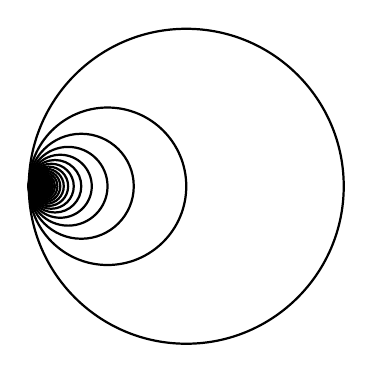
\begin{tikzpicture}
                \foreach \n in {1,...,50} {
                    \pgfmathsetmacro{\r}{2/\n}
                    \draw[thick] (\r,0) circle [radius=\r cm];
                }

                \fill ({3/50},0) circle [radius = 0.07cm];
            \end{tikzpicture}
        \end{figure}

        Veamos que el espacio topológico $B$ no es semilocalmente simplemente conexo. Para ello consideramos el punto $b=(0,0)$. Sabemos que una base de entornos de $b$ en $\bb{R}^2$ es 
        \begin{gather*}
            \beta_b = \{B(b,\veps) : \veps > 0\}
        \end{gather*}
        Al considerar la topología inducida sobre $B$ tendremos que una base de entornos será 
        \begin{gather*}
            \beta_b = \{B(b,\veps) : \veps > 0\}\cap B
        \end{gather*}
        Si fijamos un $\veps > 0$ podremos tomar un $m\in \bb{N}$ tal que $m>\frac{2}{\veps}$. Entonces tendremos que 
        \begin{gather*}
            S_m \subseteq B(b,\veps)
        \end{gather*}
        Esto se debe a que $x\in B(b,\veps) \sii d(x,b) < \veps$. Tenemos que si $y\in S_m$ entonces
        \begin{gather*}
            d(y,b) \leq d(y, (\nicefrac{1}{m}, 0)) + d((\nicefrac{1}{m}, 0), b) = \frac{1}{m} + \frac{1}{m} = \frac{2}{m} < \frac{2}{\nicefrac{2}{\veps}} = \veps
        \end{gather*}
        por lo que $y\in B(b,\veps)$. De esta forma tendremos que para todo $\veps>0$ exite al menos una circunferencia\footnote{de hecho infinitas ya que para todo $m'\in \bb{N}$ con $m'>m$ también se verificará} $S_m$ tal que 
        \begin{gather*}
            S_m \subseteq B(b,\veps)
        \end{gather*}
        Como $S_m\in B$, en particular tendremos que 
        \begin{gather*}
            S_m \subseteq B(b,\veps) \cap B
        \end{gather*}
        Por tanto, para cada entorno $U$ de $b$ tendremos que hay una circunferencia $S_m$ contenida en $U$ por lo que
        \begin{gather*}
            \pi_1(U,b) \ncong \{0\}
        \end{gather*}
        De esta forma, si consideramos la inclusión $i_U:U \to B$ tendremos que no será trivial (ya que no se puede ``cerrar'' $S_m$ en $B$).

        \item Tomamos el conjunto de $\bb{R}^3$
        \begin{gather*}
            B = \left\{ (x,y,z)\in \bb{R}^3 : 
                \begin{array}{l}
                    z=\lambda,\ \lambda \geq 0\\
                    (x,y) = \lambda(a,b),\ \text{ con } (a,b)\in \bigcup\limits_{n\in \bb{N}}S_n
                \end{array}
            \right\}
        \end{gather*}
        Donde $S_n$ es una de las circunferencias del ejemplo anterior. Esto si se analiza gráficamente es fácil ver que son un montón de conos unidos con el origen y tangentes a la recta $R = \cc{L}\{(0,0,1)\}$ y que intersecan con el plano de altura $1$ formando circunferencias tangentes al $(0,0,1)$ de la forma $S_n$.

        \begin{figure}[H]
            \centering  
            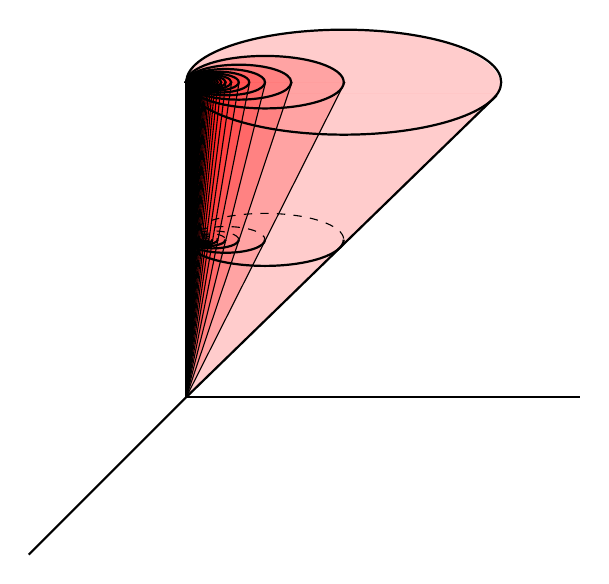
\begin{tikzpicture}
                \shorthandoff{>}


                % Relleno
                \fill[red, opacity=0.2] (0, 3.85) -- (0,0) -- (3.96, 3.85);
                \fill[red, opacity=0.2] (3.96, 3.85) arc (-10:190:2 and 0.69);

                \foreach \n in {2,...,50} {
                    \pgfmathsetmacro{\r}{2/\n}
                    \pgfmathsetmacro{\s}{2/(3*\n)}
                    \fill[red, opacity=0.2] (0, 4) -- (0,0) -- ({4.05/\n}, 4);
                    \fill[red, opacity=0.2] (0,4) arc (180:0:{\r} and {\s});
                }

                % Elipses inferiores
                \foreach \n in {1,...,50} {
                    \pgfmathsetmacro{\r}{1/\n}
                    \pgfmathsetmacro{\s}{1/(3*\n)}
                    \draw[thick] (0,2) arc (-180:0:{\r} and {\s});
                    \draw[dashed] (0,2) arc (180:0:{\r} and {\s});
                }

                % Elipses superiores
                \foreach \n in {1,...,50} {
                    \pgfmathsetmacro{\r}{2/\n}
                    \pgfmathsetmacro{\s}{2/(3*\n)}
                    \draw[thick] (\r,4) ellipse ({\r} and {\s});
                    
                }

                % Líneas contorno
                \draw[thick] (0,0) -- (3.94, 3.83);
                \filldraw[thick] (0,4) -- (0,0) -- (0.1,4);

                \foreach \n in {2,...,50} {
                    \pgfmathsetmacro{\r}{1/\n}
                    \draw (0,0) -- ({4.03/\n}, 4);
                }

                \draw[thick] (0,0) -- (0,4);
                \draw[thick] (0,0) -- (5,0);
                \draw[thick] (0,0) -- (-2,-2);

            \end{tikzpicture}
        \end{figure}

        Tenemos que $B$ es simplemente conexo por ser contráctil pero no es localmente simplemente conexo. Esto se debe a que si tomamos el punto $b=(0,1.5)$ podemos tomar un abierto de la siguiente forma:
        \begin{gather*}
            O = \left\{ (x,y,z)\in \bb{R}^3 : 
                \begin{array}{l}
                    z=\lambda,\ \lambda \in ]1,2[\\
                    (x,y) = \lambda(a,b),\ \text{ con } (a,b)\in \bigcup\limits_{n\in \bb{N}}S_n
                \end{array}
            \right\}
        \end{gather*}
        Que gráficamente será

        \begin{figure}[H]
            \centering  
            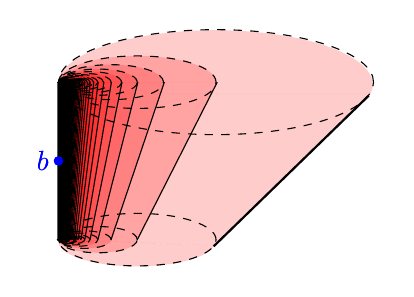
\begin{tikzpicture}
                \shorthandoff{>}

                % Punto b
                \filldraw[blue] (0,3) circle (1.5pt) node[left]{$b$};

                % Relleno
                \fill[red, opacity=0.2] (0, 3.85) -- (0,2) -- ({3.96/2}, {3.85/2}) -- (3.96, 3.85);
                \fill[red, opacity=0.2] (3.96, 3.85) arc (-10:190:2 and 0.69);
                \fill[red, opacity=0.2] ({3.96/2}, {3.85/2}) arc (-10:-184:1 and 0.32);

                \foreach \n in {2,...,50} {
                    \pgfmathsetmacro{\r}{1/\n}
                    \pgfmathsetmacro{\s}{1/(3*\n)}
                    \fill[red, opacity=0.2] (0, 4) -- (0,2) -- ({4.05/(2*\n)},2) -- ({4.05/\n}, 4);
                    \fill[red, opacity=0.2] (0,4) arc (180:0:{2*\r} and {2*\s});
                    \fill[red, opacity=0.2] (0,2) arc (-180:0:{\r} and {\s});
                }

                % Elipses inferiores
                \foreach \n in {1,...,50} {
                    \pgfmathsetmacro{\r}{1/\n}
                    \pgfmathsetmacro{\s}{1/(3*\n)}
                    \draw[dashed] (\r,2) ellipse ({\r} and {\s});
                }

                % Elipses superiores
                \foreach \n in {1,...,50} {
                    \pgfmathsetmacro{\r}{2/\n}
                    \pgfmathsetmacro{\s}{2/(3*\n)}
                    \draw[dashed] (\r,4) ellipse ({\r} and {\s});
                    
                }

                % Líneas contorno
                \draw[thick] ({3.94/2}, {3.83/2}) -- (3.94, 3.83);
                \filldraw[thick] (0,4) -- (0,2) -- (0.05,2) -- (0.07,4);

                \foreach \n in {2,...,50} {
                    \pgfmathsetmacro{\r}{1/\n}
                    \draw ({2/\n}, 2) -- ({4.03/\n}, 4);
                }

                % Punto b
                \filldraw[blue] (0,3) circle (1.5pt) node[left]{$b$};

            \end{tikzpicture}
        \end{figure}

        Y de forma análoga al ejemplo anterior, al no poder tomar ningún entorno de $b$ simplemente conexo ya que este contendrá un trozo de cono cortado, que será un cilindro topológico y por tanto no será simplemente conexo.
    \end{enumerate}
\end{ejemplo}

\begin{teo}
    Sea $B$ un espacio topológico conexo y localmente arcoconexo y fijamos un punto $b_0\in B$. Entonces las siguientes afirmaciones son equivalentes:
    \begin{enumerate}
        \item Para cada clase de conjugación de un subgrupo $H\leq \pi_1(B,b_0)$ existe un único recubridor $(R,p)$ (salvo isomorfismo), y un punto $r_0\in R$ tal que $p(r_0)=b_0$ y $H=p_*(\pi_1(R,r_0))$.
        \item $B$ tiene un recubridor universal.
        \item $B$ es semilocalmente simplemente conexo.
    \end{enumerate} 
\end{teo}